\subsection{Demoras en el arribo causados por demoras en los despegues}%
\label{sub:dep_arr_delay}

Es razonable pensar que un vuelo que se demora al despegar, va a demorarse
también al aterrizar. Se estudió la correlación entre la demora al despegue,
\texttt{DepDelay} y la demora en el momento del aterrizaje \texttt{ArrDelay}.
Se obtuvo una correlación alta, de $\rho=0.92$.

Para limpiar los datos, se utilizó un filtro de \textit{outliers} basado en una
regla escrita a mano que descarta los vuelos que se adelantan varias horas a su
hora de despegue programada. Creemos que se tratan de errores de medición.

\begin{figure}[H]
\centering
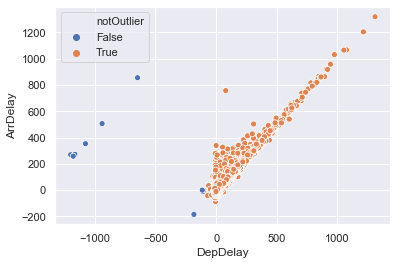
\includegraphics[width=0.5\textwidth]{img/dep_arr_delay_outliers_a_mano.png}
\caption{Relación entre la demora al despegar y la demora al aterrizar.}
\end{figure}

Se entrenó un modelo de regresión lineal entre ambas variables obteniendo un
\textsc{nrmse} de $0.00646$. La mayor densidad de puntos se encuentra sobre la
recta del modelo. Por otro lado, en el rango de
$-200\lec\mathrm{DepDelay}\leq800$ se pueden observar vuelos con un mayor
\textit{delay} al predicho por el modelo. Se propone para un futuro
experimento, añadir otros regresores para explicar dichas demoras.

\begin{figure}[H]
\centering
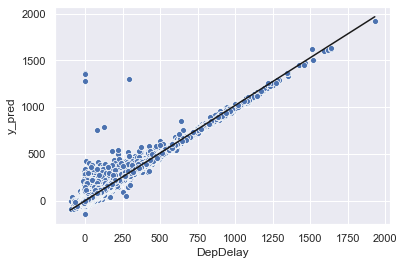
\includegraphics[width=0.5\textwidth]{img/dep_arr_delay_regplot.png}
\caption{Regresión lineal entre la demora al despegar y la demora al aterrizar.}
\end{figure}

\begin{figure}[H]
\centering
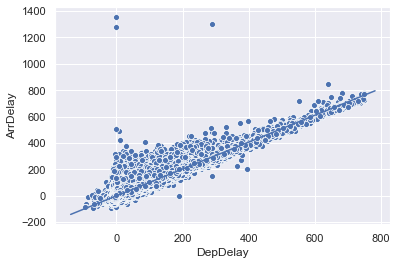
\includegraphics[width=0.5\textwidth]{img/dep_arr_delay_detalle.png}
\caption{
    Detalle de la regresión lineal para la demora al despegar y la demora al
    aterrizar en el rango $-200\lec\mathrm{DepDelay}\leq800$.
}
\end{figure}
